\documentclass[border=5mm]{standalone}
\usepackage{tikz}
\usetikzlibrary{arrows.meta, positioning, fit, shapes.symbols}

\tikzset{
  module/.style={draw, rounded corners=3pt, thick, fill=blue!6, align=center, minimum width=3.2cm, minimum height=1.4cm},
  data/.style={draw, dashed, rounded corners=3pt, thick, fill=orange!15, align=center, minimum width=3.2cm, minimum height=1.4cm},
  monitor/.style={draw, thick, rounded corners=3pt, fill=green!15, align=center, minimum width=3.0cm, minimum height=1.2cm},
  flow/.style={-Latex, thick},
  feedback/.style={-Latex, thick, dashed}
}

\begin{document}
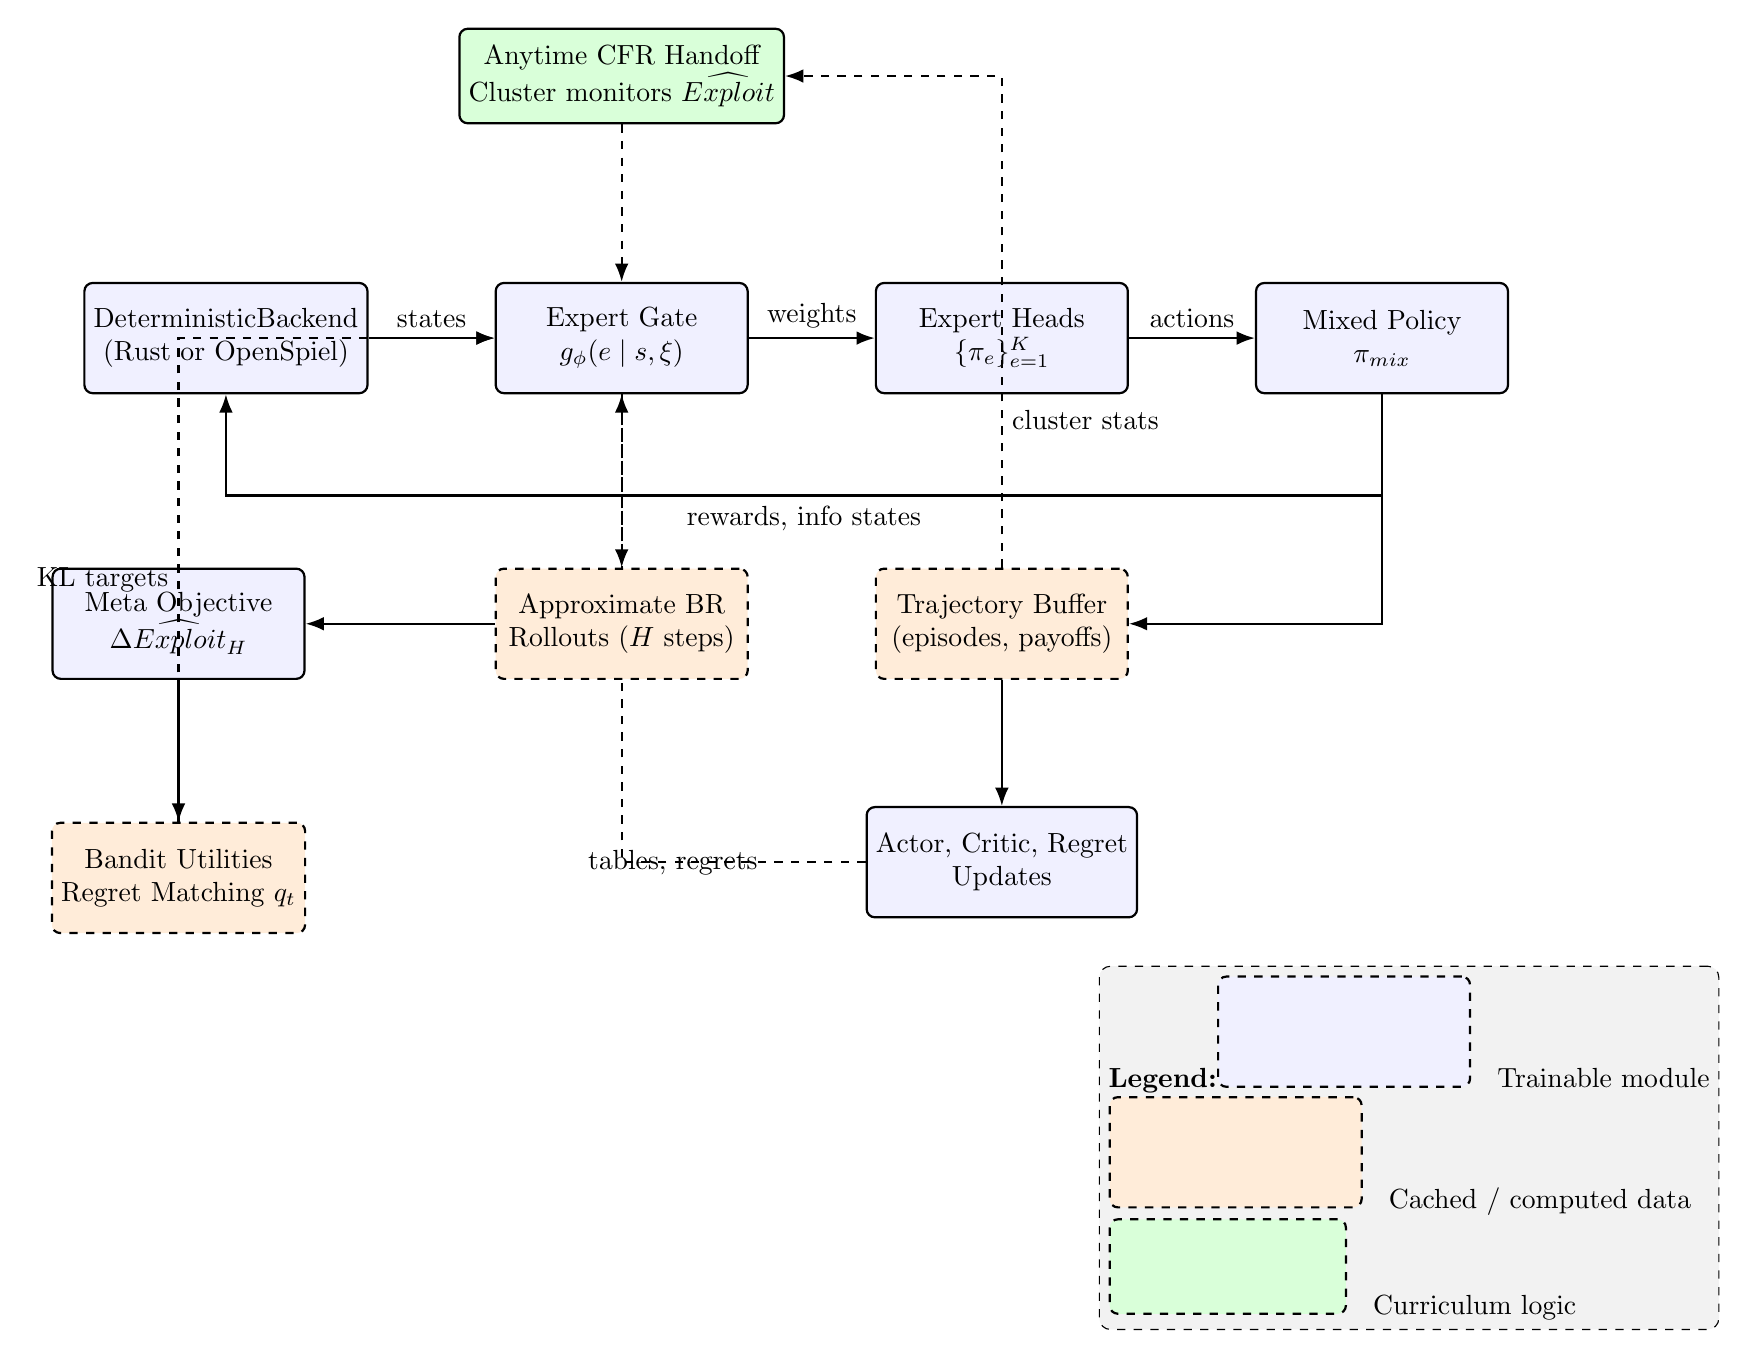
\begin{tikzpicture}[node distance=1.6cm]
  % Environment + rollout loop
  \node[module] (env) {Deterministic\newline Backend\\(Rust or OpenSpiel)};
  \node[module, right=of env] (gate) {Expert Gate\\$g_\phi(e\mid s,\xi)$};
  \node[module, right=of gate] (experts) {Expert Heads\\$\{\pi_e\}_{e=1}^K$};
  \node[module, right=of experts] (mixer) {Mixed Policy\\$\pi_{\text{mix}}$};

  \draw[flow] (env) -- node[above]{states} (gate);
  \draw[flow] (gate) -- node[above]{weights} (experts);
  \draw[flow] (experts) -- node[above]{actions} (mixer);
  \draw[flow] (mixer) |- +(0,-2) -| node[pos=0.25, below]{rewards, info states} (env);

  % Replay buffer + learners
  \node[data, below=2.2cm of experts] (buffer) {Trajectory Buffer\\(episodes, payoffs)};
  \node[module, below=of buffer] (learners) {Actor, Critic, Regret\\Updates};
  \draw[flow] (mixer) |- (buffer);
  \draw[flow] (buffer) -- (learners);
  \draw[feedback] (learners) -| node[pos=0.2, left]{tables, regrets} (gate);

  % Meta objective + BR
  \node[data, below=2.2cm of gate] (approxbr) {Approximate BR\\Rollouts ($H$ steps)};
  \node[module, left=of approxbr, xshift=-0.8cm] (meta) {Meta Objective\\$\Delta\widehat{\text{Exploit}}_H$};
  \node[data, below=1.8cm of meta] (bandit) {Bandit Utilities\\Regret Matching $q_t$};

  \draw[feedback] (gate.south) -- +(0,-0.8) -| (approxbr.north);
  \draw[flow] (approxbr) -- (meta);
  \draw[flow] (meta) -- (bandit);
  \draw[feedback] (bandit) |- node[pos=0.25, left]{KL targets} (gate);

  % CFR handoff monitor
  \node[monitor, above=2.0cm of gate] (handoff) {Anytime CFR Handoff\\Cluster monitors $\widehat{\text{Exploit}}$};
  \draw[feedback] (handoff) -- (gate);
  \draw[feedback] (buffer.north) |- node[pos=0.15, right]{cluster stats} (handoff);

  % Legend box
  \node[draw, dashed, rounded corners=4pt, fill=gray!10, align=left, below right=0.6cm and -0.5cm of learners] (legend) {\textbf{Legend:}\newline\tikz \node[module]{\phantom{xx}}; \; Trainable module\\\tikz \node[data]{\phantom{xx}}; \; Cached / computed data\\\tikz \node[monitor]{\phantom{xx}}; \; Curriculum logic};

\end{tikzpicture}
\end{document}
